\section{Limitations and Research Roadmap}
\label{sec:limitations}

The present evidence supports a precise but deliberately narrow conclusion.
This section identifies the boundaries and shows how each could be addressed
without weakening the current claim.

\subsection{Finite instance rather than universal scaling}

The numerical certificate is for the periodic $12\times12$ isotropic
Heisenberg benchmark at $T=1$ and $\eps=10^{-6}$.  Locality suggests that many
symbolic densities extend to larger tori beyond the support radius, but the
current manifest does not claim a theorem uniform in $L$, anisotropy, time, or
tolerance.  A scaling paper would require parameterized wraparound proofs,
analytic dependence of every ledger term, and certificates across a grid of
$(L,T,\eps)$ values.

\subsection{Fixed product formula and cost model}

The candidate and control use the same five-copy fourth-order Suzuki formula.
No search over modern optimized splittings is included.  Similarly, the
three-CNOT bond cost is an upper-bound compilation model, not a full
fault-tolerant resource estimate.  Native two-qubit gates, routing, parallel
depth, synthesis precision, error correction, and logical-state preparation
can change the operational optimum.  Future work should make the cost model a
pluggable certificate field and report Pareto fronts for group count, two-
qubit gates, and depth.

\subsection{Certificate size and discovery cost}

The exact D4 and D5 ledgers are large.  They are appropriate for an offline
proof artifact but not yet an interactive compiler pass.  The deep verifier is
much simpler than the generator but still scales with every listed term and
pair checked within a group.  Merkleized chunks, streaming verification,
symmetry-orbit proofs, and formally verified local rewrite kernels could
reduce storage and trust without replacing explicit evidence by an opaque
claim.

\subsection{The fivefold boundary is open}

A fivefold resource ratio would be obtained at $r=78$ because
\begin{equation}
  \frac{11{,}791}{30\cdot78+1}
  =\frac{11{,}791}{2{,}341}
  =5.036736437419906\ldots.
\end{equation}
This is arithmetic, not a 78-step error certificate.  The checked artifacts
identify three unresolved proof gates: a tighter translation-coupled D4 norm
at the 78-step budget, explicit D8 information with a delayed high-degree
tail, and a complete exact global ledger at $r=78$.  Exact D5 grouping alone
does not discharge these obligations.

\begin{figure}[t]
  \centering
  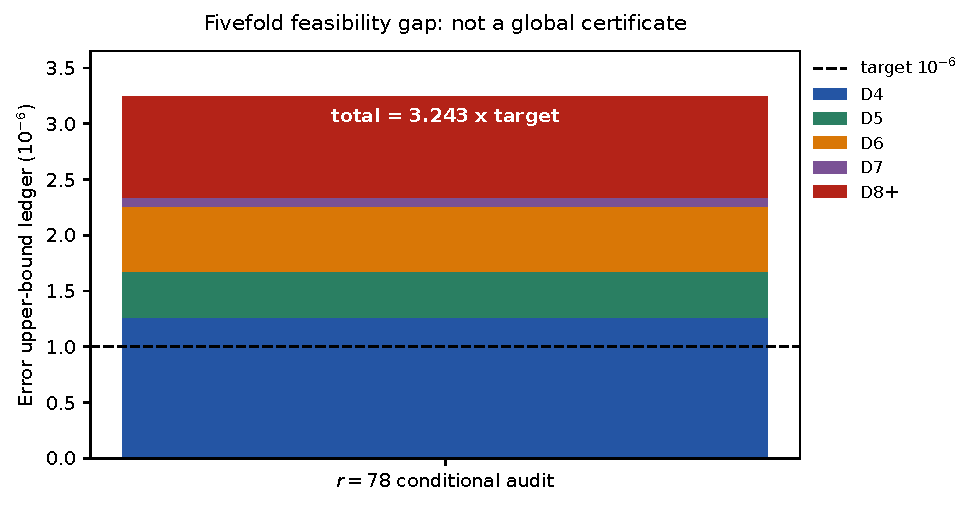
\includegraphics[width=0.8\textwidth]{figures/fivefold_gap.pdf}
  \caption{Conditional error ledger at the fivefold resource threshold.  The
  stacked value exceeds the target; $r=78$ is therefore not certified.  The
  97-step result remains the lowest accepted point of the current bound.}
  \label{fig:fivefold-gap}
\end{figure}

A disciplined optimization sequence is therefore: (1) profile the current
97-step error ledger; (2) improve the dominant D4 norm while preserving a
verifiable partition; (3) emit D8 explicitly; (4) move the geometric tail to a
higher starting degree; (5) regenerate exact contributions at 78; and (6)
accept the point only if the rational sum is at most $10^{-6}$.  GPU or HPC
parallelism can accelerate term generation and graph search, but cannot
replace the last verifier step.

\subsection{Optimality is relative to the bound}

The rejection at 96 establishes adjacent minimality only under the emitted
upper bound.  It is not a lower bound on the true operator error.  Direct
large-system matrix simulation is infeasible, and lower-bound techniques have
not been specialized here to close the gap.  Consequently the candidate may
still be physically accurate with fewer steps.  The scientific claim concerns
what can be guaranteed, not an assertion that 97 executions are necessary.

\subsection{Toward broader validation}

The most valuable next experiments are not additional decimal precision at
the current point.  They are adversarial reproductions: an independent Pauli
engine, certificates for open and periodic boundaries, anisotropic XXZ
couplings, alternate fragment orderings, and comparisons against optimized
splittings.  These tests would reveal whether the dominant gains arise from
universal compiler structure or accidental symmetries of the isotropic
benchmark.
